\chapter{Creazione del prototipo}

\section{Componenti di una web application}

Le prime fasi di tirocinio le ho concentrate sull'apprendimento dei concetti necessari per comprendere l'architettura di una web application formata principalmente da codice HTML e Javascript. La scelta del linguaggio da usare per la creazione della chat è stata univoca considerando che Javascript è ormai il linguaggio che la fa da padrone nelle moderne web app dinamiche.
Javascript è un linguaggio interpretato, che ha molto poco a che fare con il quasi omonimo Java, la prima versione venne rilasciata nel 1995 con l'obbiettivo di arricchire le pagine web aggiungendo alcune forme di dinamicità. L'utilizzo in una pagina è possibile solo se il browser del client possiede un supporto per interpretare il linguaggio, al giorno d'oggi difficilmente questa funzionalità non è presente. La popolarità di questo linguaggio permette di avere a disposizione innumerevoli librerie che consentono di semplificare lo sviluppo web permettendo di avere una portabilità del software assoluta.
Un concetto fondamentale per sviluppare software web sia lato backend sia frontend è la conoscenza del Model View Controller.
MVC \footnote{Model View Controller} è un design pattern architetturale che viene utilizzato nella programmazione a oggetti e in modo consistente nello sviluppo web, permette di separare l'architettura dell'applicativo in 3 componenti logici:
\begin{itemize}
  \item \textbf{Il Model}, componente che gestisce i dati fornendo anche i metodi per poterli utilizzare nonchè la logica e le regole dell'applicazione;
  \item \textbf{Il View} ha lo scopo di rappresentare i dati sotto forma di informazione in modo da interagire con l'utente che li visualizzerà;
  \item \textbf{Il Controller} che sulla base di richieste fornite dall'utente può modificare lo stato degli altri componenti, manipolare i dati del model o indicando una visualizzazione differente dei dati al view.
\end{itemize}
\begin{figure}[H]
 \centering
  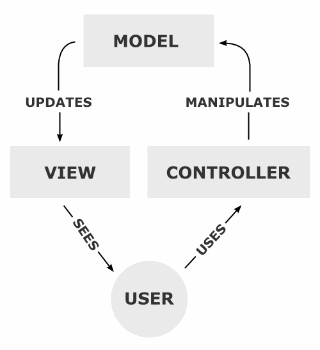
\includegraphics[width=0.5\textwidth]{img/MVC-Process.png}
 \caption{MVC}
 \end{figure}
Questa struttura viene usata principalmente per dividere la logica di business \footnote{Si definisce logica di business l'insieme delle logiche applicative di funzionamento del software} dall'interfaccia utente.
L'utilizzo di questo pattern direttamente sul client ha permesso un cambiamento importante per quanto riguarda le pagine dinamiche, cioè quello di non eseguire un redirect \footnote{Cambio di pagina} per modificare la pagina, ma eseguendo chiamate asincrone verso il server. 
Con il tempo è stato necessario fornire un framework che implementasse queste logiche riducendo i tempi di sviluppo andando a generalizzare tutti quei comportamenti classici del pattern MVC, se si parla di JavaScript senza alcun dubbio il framework più usato è AngularJs. 
Questa libreria funziona per mezzo di comandi, definiti direttive, inseriti direttamente nel codice HTML che permettono di definire le sezioni dinamiche della pagina. Il framework viene caricato all'interno della pagina attraverso l'import definito dal tag <script> in questo modo:
\begin{lstlisting}
<script
 src="https://ajax.googleapis.com/ajax/libs/angularjs/1.2.19/angular.js">
</script>
\end{lstlisting}
Questo script esegue una lettura dell'intera pagina dove saranno presenti le direttive angular che dovrà eseguire andando a modificare (o no) le sezioni della pagina che vogliamo dinamicizzare.
Lato server il più comune linguaggio usato è Java e il framework più famoso che implementa questo pattern è Spring. Come già detto Spring è un web framework open source, nato nel 2002, molto complesso che ricopre svariati campi: dalla creazione dello web server \footnote{Spring Boot}, alla manipolazione dei dati \footnote{Spring Data}, sicurezza \footnote{Spring security} e molto altro.
Considerando anche il layer database questi sono tutti i componenti da conoscere per lo sviluppo di una web application con stack Javascript e Java. 

\section{Creazione della chat}
Apprese le conoscenze base di questi strumenti ho cominciato con la stesura di una prima versione della chat testuale stand alone in Javascript. 
Una chat presuppone la comunicazione tra 2 o più soggetti, nel mio caso un soggetto è rappresentato dal cliente della banca che usa la chat e l'altro rappresentato dal bot.
I sockets sono la soluzione migliore per chat real-time con comunicazioni bidirezionali tra un client e server, questo presuppone che un client invii un messaggio e il server si prenda l'incarico di ridirezionare il messaggio al destinatario finale.
Un socket rimane attivo in ascolto su un canale di comunicazione permettendo lo scambio in input e output di messaggi e in base al tipo di messaggio trasferito verrà eseguita una azione specifica che nel caso di una chat sarà quello di stampare o inviare un messaggio. 
Un messaggio trasmesso tramite socket è caratterizzato da una chiave identificativa che definisce il tipo di messaggio inviato e dal contenuto, in questo modo è possibile trasmettere su un socket messaggi di più tipi che vengono raccolti dai consumatori dei messaggi sulla base della chiave definita. 
Per emulare questo comportamento ho usato una libreria Javascript chiamata socket.io  che tramite i metodi \textbf{emit} e \textbf{on} permettono di trasmettere il messaggio e recuperarlo, il primo serve al produttore per generare il messaggio da trasmettere nel socket mentre il secondo viene usato dal consumatore del messaggio per catturarlo.
La chat che viene richiesta però ha bisogno anche di una funzionalità in più ed è quello di permettere all'utente di parlare direttamente al bot usando la voce. Per fare questo ho dovuto usare uno strumento che trasformasse la voce catturata dal microfono in un testo, per la precisione in una stringa da poter inviare tramite il socket al controller. 
Il componente che esegue l'azione di conversione della voce in stringa viene chiamato speech recognition \footnote{Riconoscimento vocale} che esegue una traduzione da audio a testo. Per inserire questo componente nella chat ho usato una interfaccia sviluppata da Mozilla chiamata Web Speech API in cui sono presenti molte funzionalità utili per questi compiti tra cui quella di cui avevo bisogno. La funzione è SpeechRecognition che una volta configurata la lingua può essere usata. 
Per rendere visivamente usabile questo elemento nel codice HTML ho inserito un bottone che una volta cliccato attiva il microfono permettendo alla funzione di acquisire una traccia audio, quando l'utente smetterà di parlare verrà interrotta l'acquisizione e la stringa risultante sarà inviata tramite socket al componente che si occupa della comunicazione con l'intelligenza artificiale.
Il messaggio inviato all'intelligenza verrà analizzato e conseguentemente avverrà la generazione di una risposta che sarà restituita al client che procederà con la stampa del messaggio nella pagina.
Per rendere naturale la conversazione ho deciso di dare una voce al bot introducendo il procedimento inverso, anche in questo caso ho usato una funzione messa a disposizione dall'interfaccia Web Speech API chiamata SpeechSynthesisUtterance che mi ha permesso di trasformare il testo in audio dando così una voce al bot.
L'ultima cosa da fare per la parte frontend è stata una web interface minimale che permettesse di testare il funzionamento del bot, quindi c'era bisogno di:
\begin{itemize}
\item un bottone che attivasse lo speech to text \footnote{Traduzione da audio a testo},
\item una casella di testo nel caso in cui non si voglia usare il microfono,
\item 2 zone di testo dove riportare gli ultimi messaggi scambiati.
\end{itemize}
\begin{figure}[H]
 \centering
  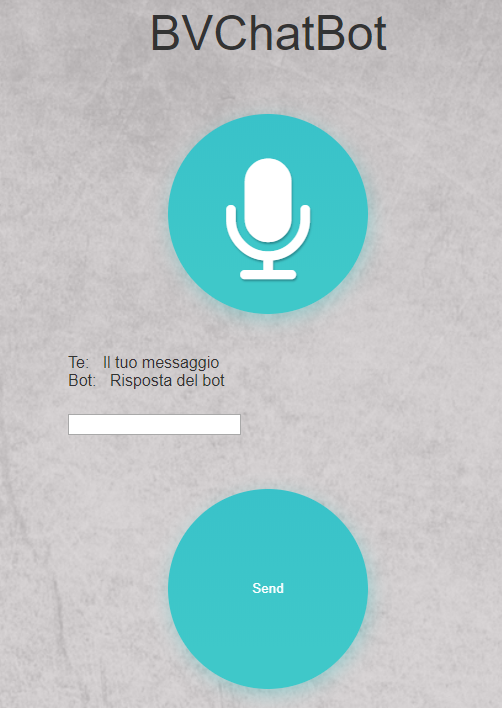
\includegraphics[width=0.4\textwidth]{img/prototype.png}
 \caption{Chat prototype}
\end{figure}

\section{Riscrittura del frontend in linguaggio typescript}

Il frontend ha avuto diverse riscritture a causa della poca esperienza in JavaScript che possedevo, l'ultima versione del prototipo è scritta in linguaggio TypeScript che ritengo molto più leggibile e facile da mantenere nel lungo tempo.
La migrazione verso JavaScript può essere complessa se si viene dal classico linguaggio orientato agli oggetti e fortemente tipizzato come Java, differentemente TypeScript favorisce un'alternativa solida con sintassi e leggibilità simile a Java.
Questo linguaggio è di per se un'estensione di JavaScript e qualsiasi script JavaScript è anche codice TypeScript valido, permettendo quindi una graduale transizione verso questa alternativa.
Lo studio e l'applicazione di questo linguaggio mi ha portato a provare diverse architetture frontend, ma quella che è risultata più efficiente è quella formata da 3 elementi principali: index.html, index.ts e script.ts.
La parte grafica rappresentata dal file index.html ha il compito di creare gli oggetti grafici e importare le librerie:
\begin{itemize}
\item \textbf{jquery} che permette la manipolazione del codice html in fase di runtime da parte di script esterni,
\item \textbf{socket.io} di cui abbiamo già parlato precedentemente.
\end{itemize}
Queste due librerie vengono usate all'interno di script.ts che ha il compito di:
\begin{itemize}
\item gestire la chat sfruttando la \textbf{comunicazione socket} ,
\item eseguire i compiti di \textbf{voice recognition e synth voice},
\item infine usando \textbf{jquery} trascrivere i messaggi scambiati tra l'utente e il bot.
\end{itemize}
La componente più importante è senza dubbio index.ts che crea il server su cui si appoggia tutto il frontend, per fare questo sono necessarie diverse dipendenze:
\begin{itemize}
\item \textbf{dotenv} con cui vengono definite delle variabili di configurazione usabili all'interno dello script consentendo una maggiore generalizzazione del prototipo,
\item \textbf{socket.io} per gestire il canale di comunicazione interno,
\item \textbf{superagent} usato per eseguire chiamate di tipo rest permettendo la comunicazione con servizi esterni,
\item  \textbf{express} framework che permette la creazione del server HTTP.
\end{itemize}
\begin{figure}[H]
 \centering
  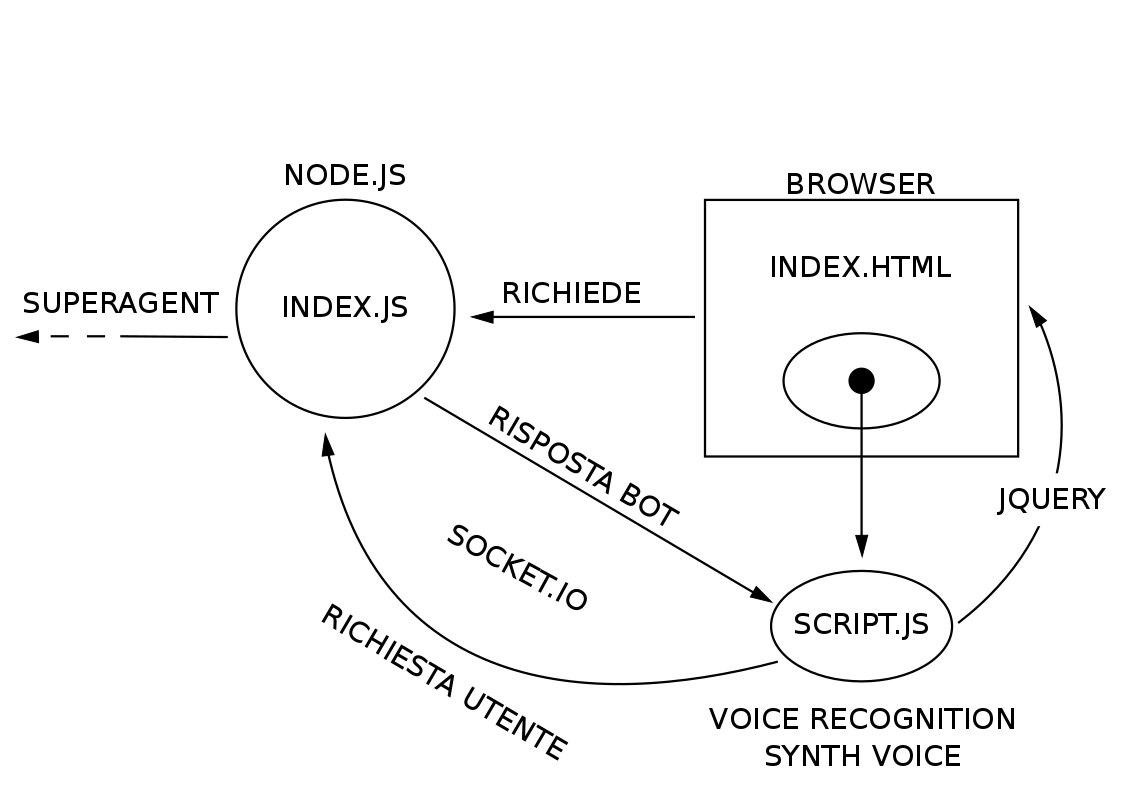
\includegraphics[width=0.8\textwidth]{img/frontend.png}
 \caption{Frontend Architecture}
\end{figure}
L'ultima dipendenza si basa su Node.js che è un motore run-time JavaScript che permette di eseguire codice JavaScript all'esterno del browser. Nel mio caso ho usato questo tool per eseguire le istruzioni fornite da express creando un server locale permettendo di accedere alla pagina index.html direttamente dal localhost.
Infine il codice scritto in linguaggio TypeScript viene transcritto utilizzando il compilatore generando effettivo codice JavaScript che viene poi eseguito dal motore Node.js rendendo usabile la chat e le sue funzionalità.

\section{Creazione dell'intelligenza artificiale}

Abbiamo trattato fino ad ora la parte relativa all'interazione con l'utente, passiamo ora alla creazione dell'intelligenza artificiale che  trasforma la chat in un chatbot. Quello di cui un chatbot ha bisogno è di analizzare la frase inviata dall'utente e generare una risposta in grado di soddisfare le richieste, sono quindi necessari 2 livelli di computazione: un'intelligenza artificiale che esegue l'analisi del testo e un'altra che in base alla storia della conversazione generi una risposta il più plausibile possibile alle richieste dell'utente.
L'analisi del testo viene definita comprensione del linguaggio naturale, in inglese \textbf{Natural Language Understanding}, cioè attribuire alla frase analizzata un intento ed estrarre da essa oggetti che possono essere utili per la generazione di una risposta.
NLU \footnote{Natural Language Understanding} è una branca dell'intelligenza artificiale che cerca metodi di analisi del testo per comprendere il significato della frase estraendo informazioni importanti. 
La generazione della risposta però non è un compito che viene esercitato dal NLU, bensì da un \textbf{Natural Language Generator} che in base all'analisi precedente riesca a determinare la miglior risposta possibile.
Questi due problemi fanno parte di un sottocampo della disciplina che studia l'intelligenza artificiale che prende il nome di Natural Language Processing, questa macro disciplina è considerata AI-Hard \footnote{Detta anche AI-Complete} questo significa che il problema non è risolvibile con un semplice algoritmo, ma è necessaria la supervisione dell'uomo per addestrare l'intelligenza a risolvere il problema specifico.
\begin{figure}[H]
 \centering
    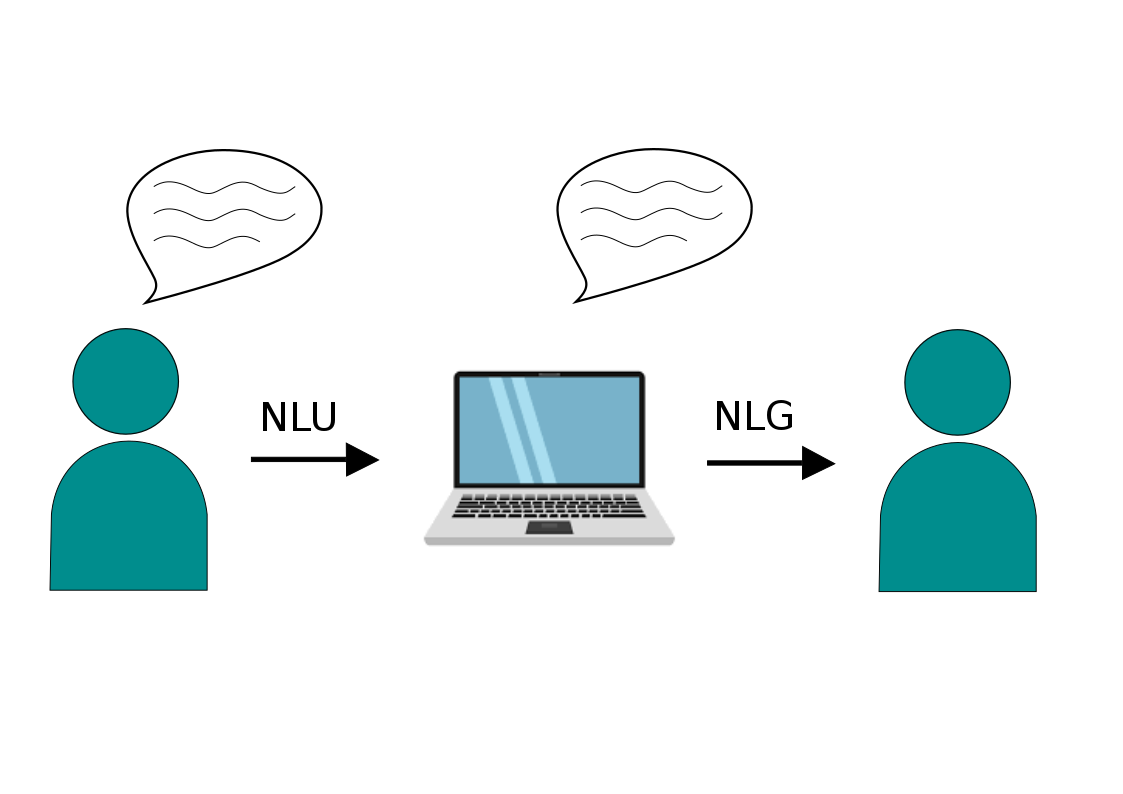
\includegraphics[width=0.6\textwidth]{img/nlu_nlg.png}
 \caption{Nlu and Nlg}
\end{figure}
Data la complessità ho ricercato uno strumento che eseguisse entrambi questi compiti e quello che mi è sembrato più vicino alle mie necessità era lo strumento chiamato \textbf{Dialogflow} \footnote{Precedentemente conosciuto come api.ai} che fornisce tutti gli strumenti necessari per quello che il bot avrebbe dovuto fare.
Dialogflow è un tool sviluppato da Google \footnote{Prima dell'acquisizione nel 2016 era sviluppato da una società chiamata Speaktoit} per la creazione di conversazioni utente macchina in linguaggio naturale che permette di sfruttare una tecnologia di questo tipo in qualsiasi contesto necessario, un punto di forza di questo strumento è l'interfaccia web molto semplificata per utenti anche alle prime armi.
Per creare un'intelligenza artificiale di questo tipo è importante creare un dataset con degli esempi chiari di conversazioni, ogni conversazione conterrà delle frasi che a loro volta conterranno delle parole chiave importanti per estrarre una risposta. Per il natural language understanding ciò di cui si ha bisogno è definire per ogni frase il suo intento e se ci sono delle entità estraibili. 
L'intento è un concetto usato per indicare l'obbiettivo della frase, utile per distinguere i vari casi che possono presentarsi durante la conversazione. 
Le entità sono invece tutti quegli elementi che costituiscono la frase che possono essere utili per comprenderne il contenuto. Ad esempio consideriamo la richiesta di un pagamento, sicuramente un'entità importante della frase è il quantitativo di soldi da versare quindi la parola che definisce questo valore sarà estratto dalla frase come elemento rilevante per la continuazione della conversazione o per l'esecuzione di un task.
La supervisione dell'uomo si basa principalmente sulla creazione di un dataset abbastanza vario e numeroso da rendere l'addestramento dell'intelligenza artificiale migliore e preciso in modo tale da creare un modello di analisi testuale efficiente. Quando si parla di creazione di un dataset si intende proprio la costruzione di conversazioni che potrebbero realmente accadere tra un operatore e un cliente, per esempio una conversazione in cui il cliente chiede la lista dei suoi conti oppure una conversazione dove invece viene eseguito un pagamento.
Il primo dataset che ho creato è formato da pochi esempi di richieste di pagamento che ho indicato con l'intento \textbf{payRequest} formato dalle possibili entità estraibili:
\begin{itemize}
\item \textbf{receiver} per estrarre il destinatario del pagamento,
\item \textbf{quantity} indica la quantità di denaro della transazione, 
\item \textbf{currency} specifica la valuta usata,
\item \textbf{account} determina il conto del cliente da cui estrarre i soldi.
\end{itemize}
\begin{figure}[H]
 \centering
  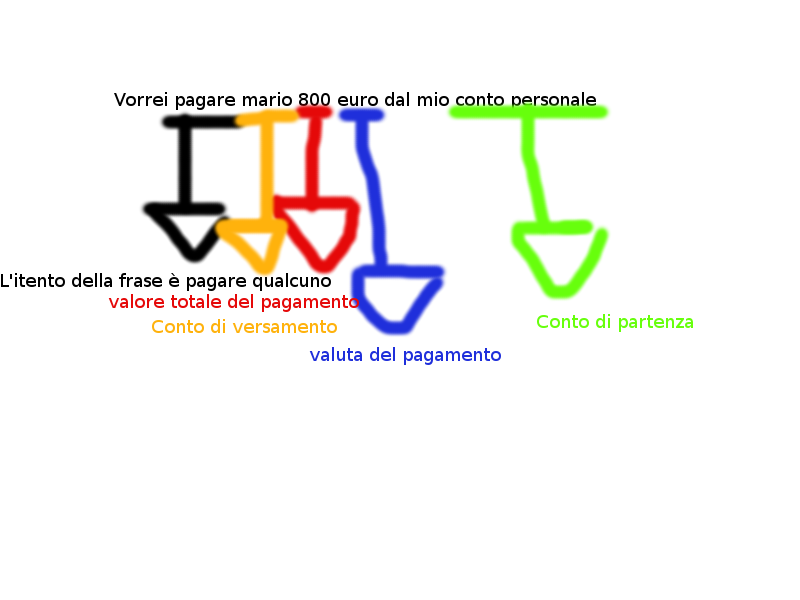
\includegraphics[width=0.9\textwidth]{img/nludatasetexample.png}
 \caption{DialogFlow example}
\end{figure}
Il motivo della creazione di un dataset ristretto mi ha permesso di integrare questo nuovo strumento con il frontend testando i metodi di conversazione e l'effettivo funzionamento della chat.
Il passo successivo sarebbe stato quello di sviluppare le richieste di pagamento effettive verso il gestionale della banca attraverso delle semplici chiamate di tipo \textbf{REST} \footnote{Protocollo di comunicazione per sistemi distribuiti}. 
Una volta presentato il prototipo funzionante sono stati segnalati alcuni problemi riguardanti la privacy dei dati degli utenti della banca.
Il problema deriva dal fatto che i dati come: iban, transazione e nome dell'utente uscivano dal range gestito dai server aziendali questo poteva generare dei problemi di privacy perchè questi dati vengono manipolati da un agente esterno, in questo caso Dialogflow.
Per risolvere questo problema ho cominciato a cercare progetti di tipo open source che racchiudessero tutte le funzionalità fornite da Dialogflow permettendo lo sviluppo in locale e che fossero efficienti alla pari con il precedente strumento.
Ho studiato diversi tools che emulassero il comportamento di Dialogflow, ma la scelta finale è ricaduta su \textbf{Rasa} sia per la sua completezza sia per la facilità di utilizzo. Rasa è un framework open source scritto in linguaggio Python diviso in 2 componenti principali: \textbf{rasa\_nlu} per eseguire le funzioni di natural language understanding consentendo quindi di classificare gli intenti ed estrarre le entità e \textbf{rasa\_core} che interrogando l'intelligenza artificiale gestisce i dialoghi con l'utente assolvendo il compito di natural language generation.
L'implementazione di queste due componenti nella realtà che dovevo realizzare comportava la creazione di un dataset molto diverso rispetto al precedente, in più lo sviluppo del bot si basa sull'implementazione di una classe Python contenente le funzionalità necessarie per completare le azioni richieste dal bot analizzando i messaggi inviati dall'utente.
Lo sviluppo del dataset necessario a rasa\_nlu per generare il modello dell'intelligenza è formato da file di configurazione in formato JSON in cui è necessario definire alcuni esempi, come fatto con Dialogflow. Un file di questo tipo è formato da 3 campi:
\begin{itemize}
\item \textbf{regex\_feature} in cui si indicano se necessario i pattern di ricerca da usare,
\item \textbf{entity\_synonyms} dove indicare il modo in cui i sinonimi debbano essere trattati
\item infine i \textbf{common\_examples} che sono il fulcro vero e proprio della definizione degli esempi.
\end{itemize}
\begin{lstlisting}
{
  "Rasa_nlu_data": {
    "regex_features": [],
    "entity_synonyms": [],
    "common_examples": []
  }
}
\end{lstlisting}
Gli entity synonyms vengono principalmente usati per sostituire l'entità estratta dalla frase con un suo sinonimo, questo viene fatto per unificare l'output delle entità estratte del test analizzato, nel mio caso ho unificato le valute monetarie europee a cui dovevo fare riferimento per il prototipo quindi euro e franco svizzero.
\begin{lstlisting}
"entity_synonyms": [
    {
      "value": "euro",
      "synonyms": ["Euro", "eur"]
    },
    {
      "value": "CHF",
      "synonyms": ["chf", "franchi svizzeri", "Franchi Svizzeri"]
    }
]
\end{lstlisting}
I common examples a loro volta sono composti da dei campi:
\begin{itemize}
\item \textbf{text} che è la stringa dove viene inserita la frase che stiamo prendendo in esame
\item \textbf{intent} rappresentante la definizione dell'intento della frase definita nel campo text
\item \textbf{entities} dove ci sono le definizioni di tutte quelle entità estratte dalla frase.
\end{itemize}
\begin{lstlisting}
"common_examples": [
    {
        "text": "Vorrei pagare Mario 800 euro dal mio conto personale",
        "intent": "payRequest",
        "entities": [{...}]
    }
]
\end{lstlisting}
Per definire una entity è necessario indicare: le posizioni di inizio e di fine della stringa, il valore effettivo che ha la stringa e infine il tipo da assegnare all'entità estratta.
Prendiamo l'esempio sopra "Vorrei pagare Mario 800 euro dal mio conto personale" da questa frase possiamo determinare con certezza che l'intento è una richiesta di pagamento, in cui ci sono diverse informazioni che possiamo estrarre: \textbf{Mario} che è il destinatario del pagamento, \textbf{800} che la quantità del versamento, \textbf{euro} che è la valuta e il conto da dove estrarre i soldi per il pagamento cioè il \textbf{conto personale} dell'utente.
\begin{lstlisting}
"entities": [
    {
        "start": 14,
        "end": 18,
        "value": "Mario",
        "entity": "destinataryAccount"
    },
    {
        "start": 20,
        "end": 22,
        "value": "800",
        "entity": "totalValue"
    },
    {
        "start": 24,
        "end": 27,
        "value": "euro",
        "entity": "currencyValue"
    },
    {
        "start": 37,
        "end": 51,
        "value": "conto personale",
        "entity": "selectedAccount"
    }
]
\end{lstlisting}
L'allenamento dell'intelligenza artificiale si baserà sui dati che abbiamo creato tramite questo dataset generando un modello da utilizzare in fase di esecuzione. Per eseguire il task di training deve essere compilato un file di configurazione in cui viene definita la lingua del linguaggio naturale e il motore che eseguirà il natural language processing.
Il file di configurazione in formato YAML è stato compilato in lingua italiana e con pipeline Spacy, libreria python per eseguire compiti di questo tipo consigliata dalla doocumentazione di Rasa nel caso in cui il numero di esempi non superi le 1000 unità:
\begin{lstlisting}
language: "it"

pipeline: "spacy_sklearn"
\end{lstlisting}
A questo punto dobbiamo configurare la parte dell'intelligenza artificiale che si occuperà di storicizzare la conversazione rendendo lo scambio di messaggi con l'utente il più realistico possibile.
Questo layer del backend, definito \textbf{CORE}, si occupa di gestire e mantenere la conversazione con l'utente eseguendo le azioni necessarie richieste, per questi scopi dobbiamo definire 3 componenti: domain, stories e actions.
La componente domain è il dominio di interesse dell'intelligenza artificiale, la cui configurazione viene creata con un file YAML in cui vengono definiti: \begin{itemize}
\item \textbf{intents} e \textbf{entities} da tracciare e riconoscere,
\item \textbf{gli slots} che sono dei contenitori di informazioni usabili e inizializzabili a run time
\item \textbf{actions} cioè le azioni che il bot può usare durante la conversazione
\item \textbf{i templates} cioè azioni default configurabili.
\end{itemize}
Il dataset relativo alle conversazioni viene definito da un set di files chiamati stories in cui sono presenti esempi vari da quelli più semplici alle conversazioni più lunghe, un esempio potrebbe essere il seguente:
\begin{lstlisting}
Utente: "Ciao bot"
Bot: "Salve"
Utente: "Arrivederci"
Bot: "Alla prossima"
\end{lstlisting}
Per riprodurre questo esempio inserendolo nel dataset è necessario usare un linguaggio di markup utile per creare testi formattati, il linguaggio più comune utilizzato in questi casi è il Markdown. L'esempio sopra tradotto in questo linguaggio diventa:
\begin{lstlisting}
# storia 1
* inizio_conversazione
    - risposta_inizio_conversazione
* fine_conversazione
    - risposta_fine_conversazione
\end{lstlisting}
La prima riga, il cui primo carattere è \textbf{\#}, rappresenta una descrizione della storia e non ha un riscontro effettivo sul training, ma è solo utile a livello di sviluppo per aiutare a differenziare le varie storie che vengono scritte o inserite nel dataset.
Le due righe successive con primo carattere \textbf{*} e \textbf{-} sono rispettivamente la definizione dell'intento della frase inviata dall'utente e l'azione di risposta del bot corrispondente.
Determinare delle stories il più realistiche possibili permette al bot di essere coerente con l'andamento della conversazione anche quando questa non segue i binari definiti nel dataset con cui il modello è stato generato.
Infine alla componente actions corrispondono le modalità con cui il bot può rispondere, ma non solo perchè all'interno di ogni action possono essere eseguite delle istruzioni aggiuntive. Nel nostro caso saranno richieste al server che si occupa della monetica per esempio un pagamento o recuperare la lista dei conti correnti.
A livello di codice le actions sono definite tramite l'implementazione di classi Python che estendono l'interfaccia Action del framework \textbf{rasa\_core}.
L'implementazione di questa classe deve definire 2 metodi principali: 
\begin{itemize}
    \item \textbf{name} che deve ritornare una stringa con il nome dell'azione a cui il modello dovrà fare riferimento 
    \item \textbf{run} che è l'implementazione dell'azione.
\end{itemize}
Il metodo run assume 3 parametri che potranno essere usati all'interno della definizione del metodo: 
\begin{itemize}
    \item \textbf{dispatcher} che è usato per mandare messaggi di risposta all'utente, 
    \item \textbf{tracker} dove vengono mantenute le informazioni della conversazione con l'utente,
    \item \textbf{domain} in cui sono contenute tutte le informazioni di dominio del bot.
\end{itemize}
\begin{lstlisting}
class ActionGreetings(Action):

    def name(self):
        return "ActionGreetings"

    def run(self, dispatcher, tracker, domain):
        dispatcher.utter_message("Ciao")
        return []
\end{lstlisting}
Non c'è molto da dire per quanto riguarda il training dell'intelligenza, essendo un tool completo Rasa mette a disposizione anche gli strumenti per generare entrambi i modelli necessari. Basterà quindi indicare alcune configurazioni che dovrà utilizzare durante l'esecuzione del processo di training.
Per quanto riguarda il NLU dovremo indicare principalmente: la path del config dove abbiamo definito la lingua e lo strumento di machine learning da usare, dove si trova il dataset e il nome del modello da restituire in output.
\begin{lstlisting}
python -m rasa_nlu.train  \
    --config nluModelConfig.yml \
    --data data/ \
    --project current \
    --fixed_model_name nlu \
    --path models/
\end{lstlisting}
Allo stesso modo l'esecuzione del training del CORE avrà bisogno di informazioni riguardanti la posizione del domain e delle stories, inoltre il numero di epochs cioè il numero di iterazioni che il processo di machine learning dovrà eseguire.
\begin{lstlisting}
python -m rasa_core.train \
    -d payment_domain.yml \
    -s stories/payment_stories.md \
    -o models/current/core \
    --epochs 300
\end{lstlisting}
L'inizializzazione del server avrà bisogno dei due modelli creati e un indirizzo più una porta in cui rimanere in ascolto di richieste esterne, inoltre ho definito anche un token per rendere la comunicazione più sicura.
\begin{lstlisting}
python -m rasa_core.server \
    -d models/current/core \
    -u models/current/nlu \
    --cors 'http://localhost:8080' \
    --auth_token securitytoken
\end{lstlisting}

\section{Aggiornamento Frontend}
Per poter comunicare con il nuovo server è necessario modificare alcune variabili del frontend quali: \textbf{l'indirizzo del server}, \textbf{la porta} e \textbf{il token} usato per la comunicazione con il server relativo all'intelligenza artificiale.
Per rendere più semplice la manutenzione di queste informazioni, ho utilizzato un file di configurazione chiamato .env in cui vengono contenute tutte le informazioni relative al backend Rasa:
\begin{lstlisting}
SERVER_IP_RASA=127.0.0.1
SERVER_PORT_RASA=5000
TOKEN_RASA=securitytoken
\end{lstlisting}
Per fare in modo di usare in maniera semplice e veloce queste configurazioni creiamo una classe chiamata Settings e una volta importato il file usando dotenv viene istanziato un oggetto che avrà le stesse proprietà importate. In questo modo in ogni momento a runtime potrà essere usato per ottenere informazioni riguardanti il server dove si trova l'intelligenza artificiale.
La comunicazione con il server avviene grazie alla definizione di una classe chiamata \textbf{ComunicationRasaManager} implementata nel file index.js in cui è definita la funzione \textbf{questionAndAnswer} responsabile dell'invio e della ricezione dei messaggi con il server, questa funzione assume 5 argomenti:
\begin{itemize}
\item l'oggetto socket che si occupa del canale di comunicazione interno al client,
\item il messaggio che deve essere inviato al server,
\item lo URL relativo all'indirizzo di provenienza del server,
\item l'identificativo univoco dell'utente,
\item e infine il token che rappresenta la chiave per poter aver accesso al server.
\end{itemize}
L'implementazione del metodo esegue una chiamata REST di tipo POST con il body contenente il messaggio dell'utente verso il componente NLU del server Rasa che si occupa dell'analisi del testo. L'intelligenza analizzerà il messaggio estraendo le entità e l'intento, queste informazioni vengono poi inviate al componente NLG che determinerà il messaggio di risposta che viene infine inviato come risposta al chiamante. Il messaggio ricevuto da index.js viene poi inviato tramite socket al componente frontend script.js che si occuperà finalmente di manipolare i componenti grafici della pagina in modo da visualizzare il messaggio e continuare la conversazione.
Tutto questo è valido nel caso ideale cioè quando tutte le chiamate restituiscono una risposta corretta o se il server non ha trovato degli errori a runtime. Ho cercato di prevenire i fallimenti lato frontend rendendo stabile quanto possibile la chat. 

\section{Sistema di pagamento vocale}

La parte di setup della conversazione a questo punto si può dire conclusa, rimane da instaurare il layer di comunicazione tra il backend Rasa e il backend che si occupa di monetica in modo tale da poter eseguire le operazioni necessarie per rispettare ogni richiesta fatta dal cliente durante la conversazione. Considerando il contesto prima di eseguire una qualsiasi operazione come una transazione sono necessarie le credenziali e il consenso dell'utente. Il prototipo però non poteva accedere direttamente alle informazioni di un cliente reale quindi è stato creato un utente fittizio nel database di test dell'azienda.
Questo però non è bastato dato che l'intelligenza artificiale viene considerata come un agente esterno al server di monetica quindi viene bloccata ogni tipo di operazione. Per rendere possibile eseguire delle richieste è inevitabile passare dal lato utente e abilitare il server Rasa ad acquisire i dati, manipolarli e richiedere operazioni per conto del cliente.
Per fare questo dobbiamo prendere in considerazione che ogni utente è protetto da una doppia autenticazione e solo dopo la seconda autenticazione viene rilasciato il token per eseguire le operazioni utili. Il token è un identificatore di sessione e fintanto che la sessione rimane attiva questo rimane utilizzabile, una volta che scade deve essere ricreato costringendo l'utente a rieseguire l'autenticazione. Può essere interpretato come una chiave di accesso alle informazioni dell'utente, una volta ottenuto l'identificatore tutto viene concesso e questo è il motivo per cui è protetto da più strati di sicurezza.
Una protezione così rigida impedisce l'acquisizione di questo token in maniera automatica di conseguenza le informazioni del cliente risultano inaccessibili, per risolvere questo problema è stato deciso di non modificare questo livello di sicurezza, ma per il momento di inserire manualmente questa chiave per ogni nuova conversazione.
Per inserirlo viene usato uno slot \footnote{Una feature del framework che permette di avere una temporanea persistenza dei dati} associato alla conversazione in questo modo è possibile salvare la chiave e usarla al momento di una qualche operazione bancaria, fintanto che la conversazione non si conclude e gli slots vengono svuotati.
L'impostazione di questa variabile viene fatta tramite l'interfaccia REST messa a disposizione da Rasa tramite la quale viene inviato il token e salvato in un apposito slot relativo alla conversazione. 
\begin{lstlisting}[caption={Comando da eseguire per valorizzare gli slots}]
curl -XPOST \
    <indirizzo>:<porta>/conversations/default/tracker/events \
    -d '[{ "event": "slot", \
        "name": <nome token>, \
        "value": <valore del token> }]'
\end{lstlisting}
Possiamo concludere dicendo che ad ogni conversazione quindi sono associate due caratteristiche fondamentali che sono la chiave di sessione e l'identificatore della storia della conversazione, con questi due elementi è possibile associare in modo univoco le operazioni richieste dall'utente che sta utilizzando il chatbot, in questo modo se necessario è possibile avere anche un sistema di tracciamento delle conversazioni di ogni utente.
Avendo tutto il necessario è stato possibile completare le actions utili per eseguire una storia di conversazione di base: richiesta dei conti correnti, scelta del conto corrente da usare, totale del conto selezionato, pagamento, conferma o disdetta del pagamento.
\begin{figure}[H]
 \centering
    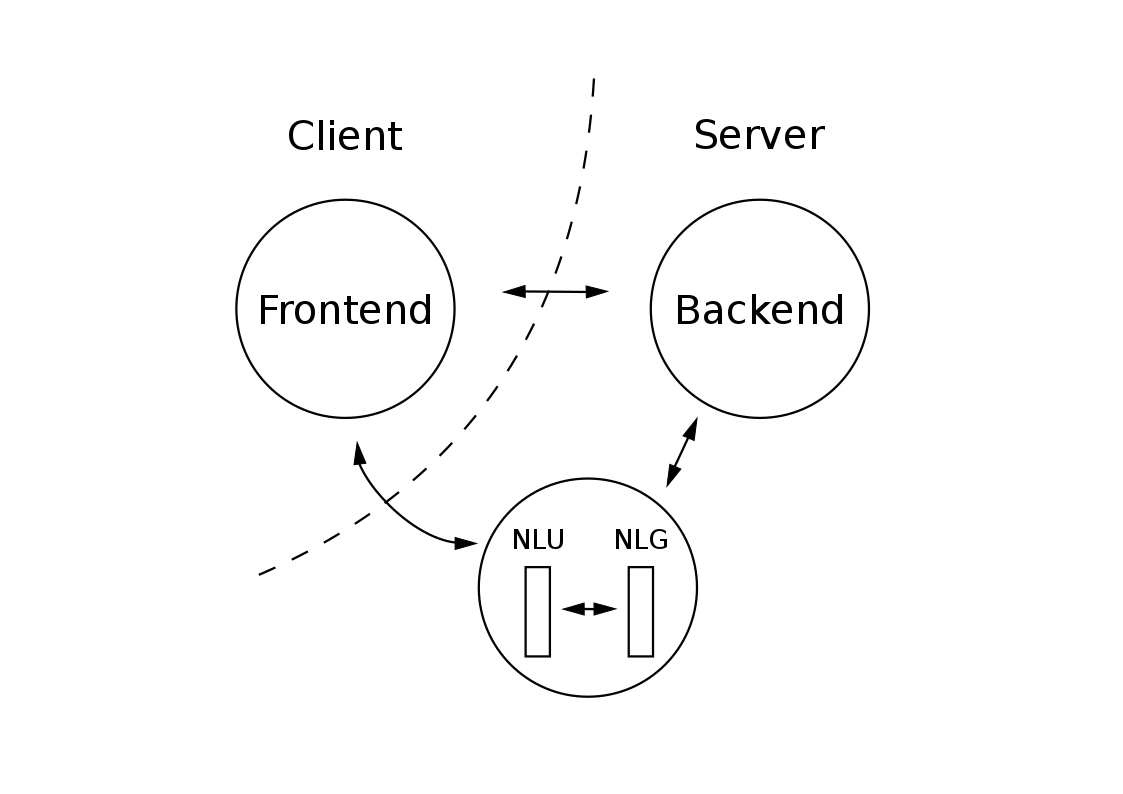
\includegraphics[width=0.9\textwidth]{img/last_architecture.png}
 \caption{Architecture}
\end{figure}

\section{Funzionamento e esecuzione}

Il prototipo stand-alone è a questo punto completo in quanto tutti i componenti sono collegati tra di loro e funzionano come richiesto. Per poterlo eseguire sono necessarie molte dipendenze sia per la parte frontend che per la parte relativa all'intelligenza artificiale.
Il frontend ha necessità di usare \textbf{Node.js} e \textbf{npm}, il primo usato per la creazione del server web della chat mentre il secondo è un package manager usato per installare i moduli javascript e typescript usati.
Tutte le dipendenze vengono indicate in un file in formato json chiamato package, tramite questo file è possibile rendere lo sviluppo della chat portabile e rigido per quanto riguarda le versioni dei pacchetti usati. Per installare l'ambiente di sviluppo basterà eseguire il comando di installazione di npm che provvederà a creare una directory locale al progetto contenente tutti i moduli previsti dal file package.
A questo punto è possibile utilizzare il transcriber typescript per generare i file javascript a partire dagli script che abbiamo sviluppato, questo serve per poter usare node che esegue solo codice javascript.
Node eseguirà index.js che utilizza il web framework \textbf{Express} per creare un web server rendendo accessibile la pagina index.html.
Passando al layer del backend utilizziamo un interprete di linguaggio \textbf{Python} che quindi deve essere installato per eseguire i compiti di training dell'intelligenza e creazione del server web, tutte le dipendenze anche in questo caso sono mantenute all'interno di un file chiamato requirements che contiene nome e versione di ogni modulo. L'installazione viene messa a punto dal package installer \textbf{pip}, che esegue un parse del file requirements e procede con l'installazione dei vari componenti.
Le dipendenze del backend sono tante: 
\begin{itemize}
    \item \textbf{Flask} che è il framework usato da rasa per mettere in piedi lo web server, 
    \item \textbf{Spacy} usata per i compiti di processing del linguaggio naturale, 
    \item \textbf{Tensorflow} per i train dell'intelligenza artificiale, 
    \item infine le componenti core di Rasa e tutti i micro pacchetti utilizzati da queste macro dipendenze.
\end{itemize}
Una volta importate queste dipendenze si deve scaricare il dizionario della lingua italiana usato durante il training del modello e durante l'esecuzione effettiva dell'intelligenza, di default altrimenti viene importato il dizionario inglese.
Una volta conclusa questa prima fase di installazione si può procedere con la fase di train dell'intelligenza artificiale che è suddivisa come già detto in 2 parti generando quindi 2 modelli differenti: uno per il natural language understanding e uno per il natural language generation, indicativamente per eseguire entrambi gli addestramenti vengono impiegati tra i 20 e i 30 minuti \footnote{i tempi variano molto in base alla macchina in cui viene eseguito l'addestramento}.
Concluso il training dei componenti è possibile unire tutti i componenti ed eseguire il web server, rendendo accessibile e usabile l'intero sistema concludendo così la creazione di un prototipo funzionante.
